\section{Motivation}\label{sec:motivation}

% Overview

To use stream ciphers for performant FDE, StrongBox leverages two key insights:
1) the overwrite-averse \emph{append-mostly} behavior of Log-structured File
Systems (LFS) and 2) the division of the backing store into discrete same-size
metadata-managed units \emph{above the block I/O layer} referred to as
\emph{nuggets}. When the rare overwrite does occur during I/O, StrongBox
modifies the cipher keystream or \emph{rekeys} the affected nugget(s) to prevent
a confidentiality violation.

This approach naturally leads to transitioning individual nuggets between any
cipher during runtime. This is because 1) encryption and decryption of nuggets
is compartmentalized; nugget-level operations occur independently of one another
and 2) all rekeying operations end up committing data to "empty"
(\ie{initialized with random data}) space on the backing store.

We can build on this behavior by abstracting the rekeying process out into a
\emph{re-ciphering} process, whereby the key \emph{and the cipher used to
encrypt/decrypt the nugget} can both be switched at runtime. This allows us to
trade off between different ciphers and their characteristics dynamically,
whereas prior work can only accomplish a static tradeoff at compile time or
filesystem initialization.

\subsection{Quantifying the Security Dimension}

To reason about trading off the security guarantees provided by various ciphers,
the strength of these guarantees must be quantified through scoring. For our
purposes, we arrived at three key features that, when scored, give us a useful
quantification of cipher security (see: \tblref{security-quant}).

\begin{itemize}

 \item \emph{Output randomization.} A cipher that exhibits output randomization
 can output ciphertext non-deterministically given the same input, which is
 extremely useful for FDE\@. This is a binary feature in that a cipher either
 outputs deterministically or it does not. A cipher with output randomization
 scores a 1 for this feature while a cipher without it scores a 0.

 \item \emph{Resistance to cryptanalysis.} A cipher that is resistant to
 cryptanalysis can resist theoretical cryptanalytical attacks such as
 known-plaintext and chosen-plaintext attacks, offline key-guessing attacks, et
 cetera. Scores for this feature range from 0 to 1, where 0.5 represents
 standard resistance to cryptanalysis for stream ciphers in the general case\@.

 \item \emph{Round count vs standard.} The ciphers we examine in this research
 are all constructed around the notion of \emph{rounds}, where a higher number
 of rounds implies a stronger confidentiality guarantee. This feature represents
 how many rounds the cipher executes compared to the accepted "standard" round
 count for that cipher. For instance, ChaCha8 is a reduced round version of the
 standard ChaCha20. Variants are distributed evenly from 0-1. For instance,
 ChaCha8 scores 0, ChaCha12 scores 0.5, and ChaCha20 scores 1\@.

\end{itemize}

\begin{table}[]
   \begin{tabular}{@{}lllll@{}}
   \toprule
   \textbf{Cipher} & \textbf{OR} & \textbf{CR} & \textbf{RR/RK} & \textbf{Rank} \\ \midrule
   ChaCha8         & 0           & 0.5         & 0              & 0.5           \\
   ChaCha12        & 0           & 0.5         & 0.5            & 1             \\
   ChaCha20        & 0           & 0.5         & 1              & 1.5           \\
   Salsa8          & 0           & 0.4         & 0              & 0.4           \\
   Salsa12         & 0           & 0.4         & 0.5            & 0.9           \\
   Salsa20         & 0           & 0.4         & 1              & 1.4           \\
   AES128-CTR      & 0           & 0.5         & 0              & 0.5           \\
   AES256-CTR      & 0           & 0.5         & 1              & 1.5           \\
   HC128           & 0           & 0.5         & 0              & 0.5           \\
   HC256           & 0           & 0.5         & 1              & 1.5           \\
   Rabbit          & 0           & 0.4         & 1              & 1.4           \\
   Sosemanuk       & 0           & 0.4         & 1              & 1.4           \\
   Freestyle (F)   & 1           & 1           & 0              & 2             \\
   Freestyle (B)   & 1           & 1           & 0.5            & 2.5           \\
   Freestyle (S)   & 1           & 1           & 1              & 3             \\
   AES128-XTS      & 0.2         & 0.5         & 1              & 1.7
   \end{tabular}
   \caption{\TODO{Table caption goes here.}}
   \label{tbl:security-quant}
\end{table}

\subsection{Statically Trading off Energy/Latency for Security}

\begin{figure}[ht]
 \centering
  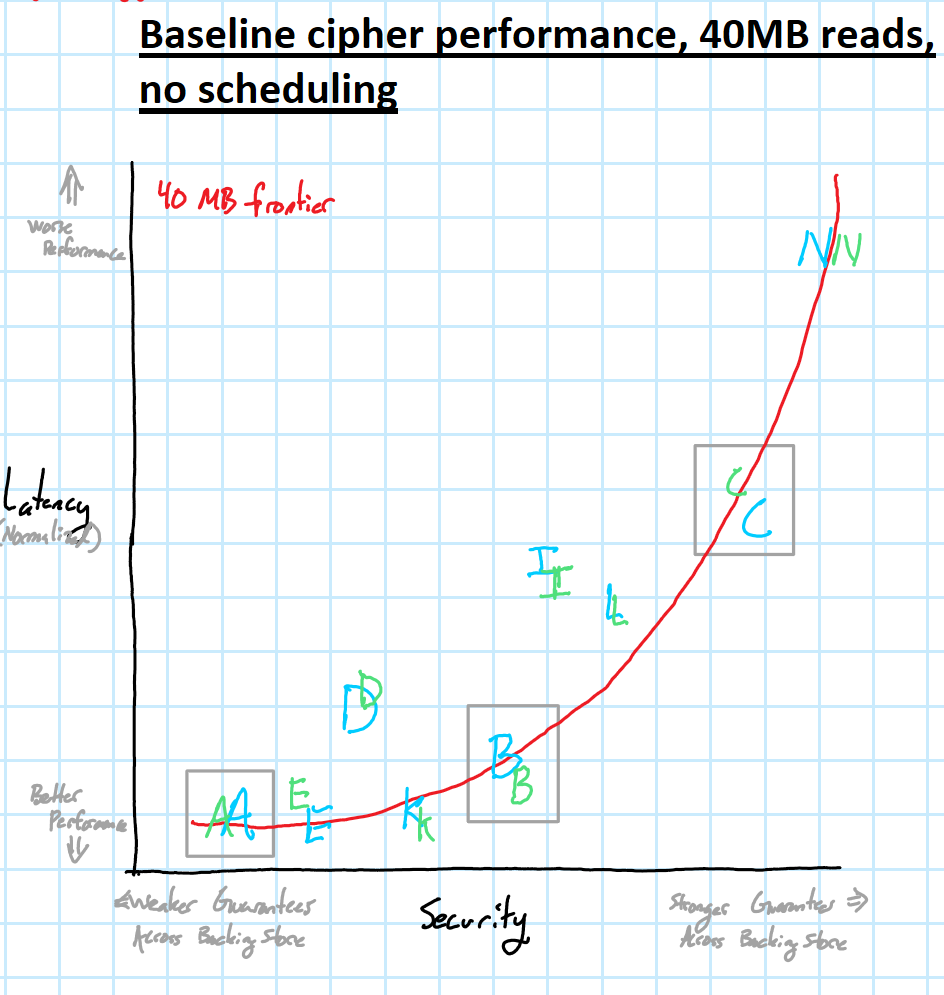
\includegraphics[width=0.8\linewidth]{drawn/1.png}
   \caption{\TODO{Caption goes here}\TODO{No curve in this version!}}\label{fig:40mb-read}
\end{figure}

\figref{40mb-read} shows the security versus I/O latency static
tradeoff between different stream ciphers under StrongBox when completing a 40MB
read of encrypted storage. The experiment was performed on an ARM big.LITTLE
Exynos Octa processor, which is similar to the processors used in the Samsung
Galaxy line of phones and other devices. \TODO{In the LaTeX figure, pareto
frontier is X while other results are some other shape. Explain this here.}

Ciphers with relatively stronger security guarantees result in higher latency
for I/O operations while ciphers with relatively weaker security guarantees
result in lower latency.

\begin{figure}[ht]
 \centering
  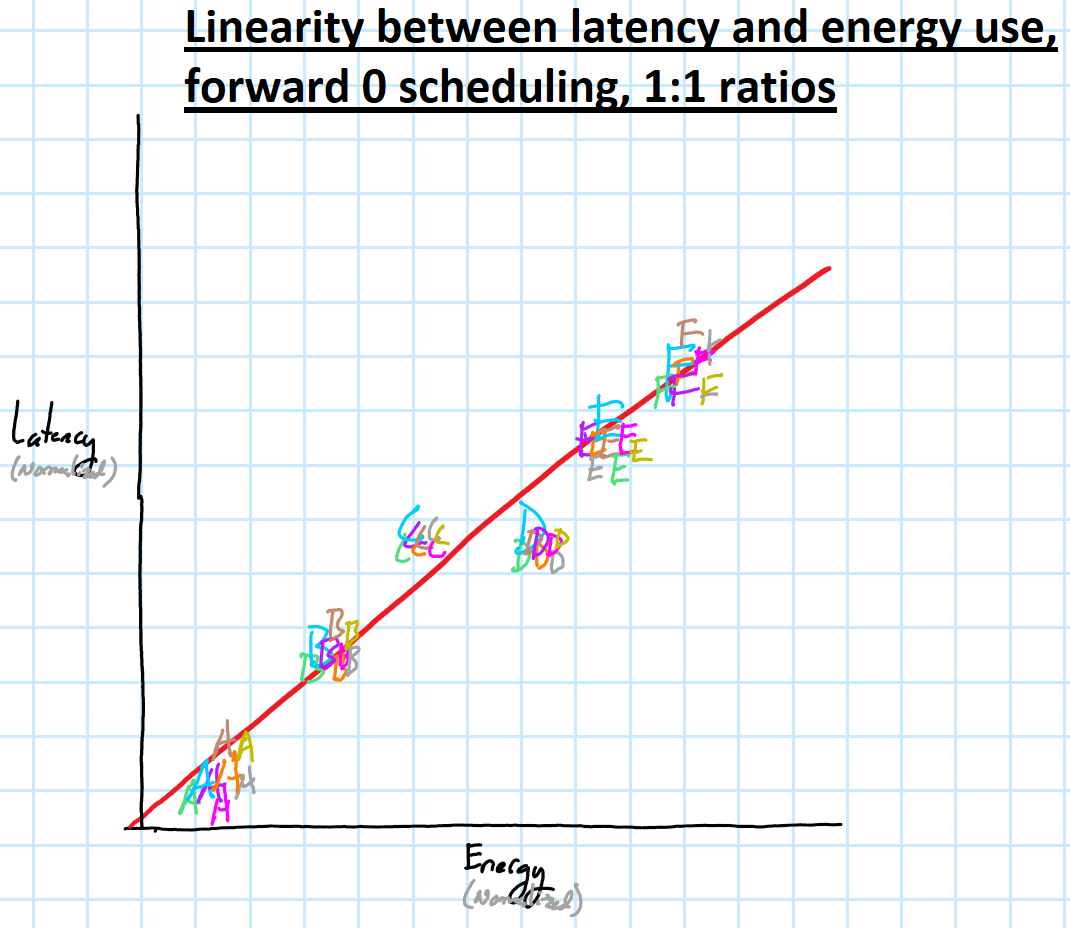
\includegraphics[width=0.8\linewidth]{drawn/5.png}
   \caption{\TODO{Caption goes here}}\label{fig:energy-latency-linearity}
\end{figure}

\figref{energy-latency-linearity} shows that, for the stream ciphers included in
our experiments, there is a linear relationship between cipher performance and
total energy used during the I/O operation.

With prior work, \TODO{we could cite other filesystems and storage layers here
other than just StrongBox, such as ZFS, dmcrypt?} cipher configuration is made
statically at compile time or at filesystem initialization. This forces
developers and end-users to choose a configuration that works best in the most
general case and stick with it, even if a different configuration becomes more
optimal at a later point. The only way to switch ciphers when a new
configuration becomes more optimal is to recreate the entire underlying
filesystem, which is rarely desirable. \TODO{This paragraph should be fleshed
out more?}

\subsection{Dynamically Trading off Energy/Latency for Security}

\begin{figure}[ht]
 \centering
  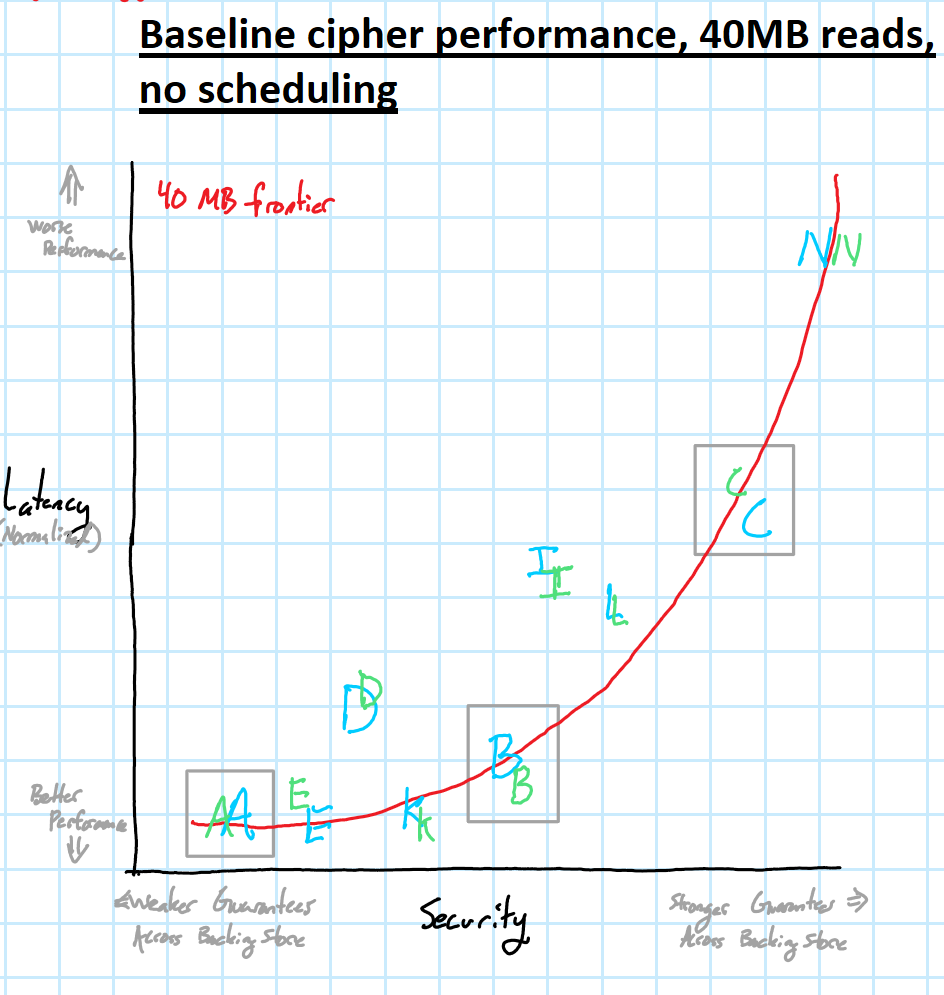
\includegraphics[width=0.8\linewidth]{drawn/1.png}
   \caption{\TODO{Caption goes here}\TODO{Include pareto curve in this version??}}\label{fig:40mb-read-with-forward}
\end{figure}

But what if our system didn't have to sit at a static configuration point, even
when another configuration became more optimal in context? This motivates the
need for some dynamic mechanism to navigate this tradeoff space online at
runtime. More than just switching between static configuration points, such a
mechanism would allow the system to dynamically switch to otherwise unreachable
configurations along the pareto frontier curve between and including the
discrete points achievable with prior work depending on the needs of the system
at that moment in time. In \figref{40mb-read-with-forward}, we see examples of
such points. \TODO{\figref{40mb-read-with-forward} will show configuration
points along pareto curve and differentiate between static points and dynamic
points with shapes versus the other version of this chart (above) which shows
none of this}

% Or should this be a new section?
Two examples motivating this mechanism follow.\\

\noindent
\textbf{Temporal switching: streaming video with a curtailed energy budget}

\TODO{Are we stepping on the use case section with this?}

Suppose we were streaming a video stored our mobile device to a WiFi connected
television or projector. We want to store video and other data on our device as
securely as possible, so we chose to initialize the system at configuration
point offering very strong security. \figref{energy-latency-linearity}
correlates stronger security guarantees with greater total energy use, meaning
our device is using a lot more energy to facilitate FDE at this configuration
point.

Eventually, our device determines its remaining battery life is too low and
enters an energy saving mode. With a traditional filesystem, we are stuck with
our static high-energy configuration chosen at system initialization.

However, with the ability to operate at points along the pareto frontier (c.f.
\figref{40mb-read-with-forward}), even at points between the discrete
configurations available to prior work, a context-aware system can switch to a
configuration that trades the security of the portions of storage that are being
used to stream the video so that we stay within our curtailed energy budget.

When we return to a non-curtailed energy budget, the system can return to its
more secure configuration dynamically, allowing the cipher strength of the
backing store to eventually recover without having to recreate the entire
underlying filesystem.\\

\noindent
\textbf{Spatial switching: securing a massive multi-cipher document}

\TODO{Are we stepping on the use case section with this?}

Suppose a large organization that is working on a document with hundreds of
gigabytes of data. The organization is decentralized, so this document must pass
back and forth among several disparate parties who are constantly encrypting and
decrypting certain sections of it to work on. Of course, this document is the
target of frequent brute force, supply chain, and other confidentiality
violating attacks by powerful adversaries with unknown and potentially unlimited
means at their disposal. The confidentiality of the document must never be
violated, so it must be encrypted. However, some tiny amount of the data
dispersed throughout the document is \emph{highly} sensitive; and while a
confidentiality violation of the wider document would be embarrassing, a
confidentiality violation of this very sensitive data would very likely destroy
the organization in its entirety.

With prior work, this organization is limited to static configurations that
generally fall within two camps: 1) encrypt the entire document with a cipher
providing the strongest security guarantees possible to protect the small amount
of highly sensitive data, which would add an unacceptable overhead to the
frequent encryption and decryption operations of the organization during I/O or
2) encrypt the entire document with a cipher providing the least amount of
latency during I/O, which could potentially leave the organization vulnerable to
its adversaries.

However, with the ability to operate at points between the discrete
configurations available to prior work, a dynamic system can encrypt highly
sensitive portions of the backing store with the cipher with the strongest
security guarantees while allowing the rest of the document to be encrypted with
the standard cipher so as to not unduly burden the employees of this
organization as they operate on the document.
